\chapter{LAPORAN}
\section{TUGAS TEORI}
\begin{enumerate}
	\item sejarah python\\
	Python dibentuk oleh Guido van Rossum di  Centrum Wiskunde \& Informatica (CWI) di Belanda pada awal tahun 1990. 	Bahasa pemrograman ABC merupakan inspirasi dari adanya bahasa python yang digunakan saat ini. Guido merupakan penulis utama dari bahasa python sampai sekarang ini, walaupun pada kenyataannya python bersifat open source sehingga setiap orang dapat turut berkontribusi dalam mengambangkan bahasa python
	\item perbedaan python 2 dan python 3\\
Python merupakan bahasa pemrograman yang terbilang paling sederhana dibandingkan dengan bahasa pemrograman yang lainnya. oleh karenanya bahasa python banyak digunakan oleh perusahaan-perusahaan besar karena keefektif dan keefisiensiannya, di samping itu karena sederhananya bahasa pemrograman ini, maka python mudah dipelajari dan dipahami oleh berbagai kalangan.\\
Saat ini, ada 2 jenis python yang beredar di masyarakat, yakni python versi 2 dan python versi 3. Python versi 2 merupakan versi yang lebih banyak digunakan di kalangan pengembang atau developer dan di lingkungan produksi, sedangkan Python versi 3 merupakan pengembangan dari versi 2. Sehingga, Python 3 memiliki lebih banyak fitur di dalamnya. Penggunaan antara keduanya pun terbilang hampir mirip. Akan tetapi terdapat beberapa perbedaan yang ada di antara keduanya, antara lain :\\
	\begin{itemize}
		\item Untuk membuka python 2, kita hanya diperlukan mengetik "python" saja. Sedangkan untuk membuka python 3, kita harus menggunakan perintah python3
		\item Sintaks yang digunakan untuk mencetak teks\\
		Pada python 2, sintaks yang digunakan ialah :\\
			\begin{enumerate}
			\item print "teks yang ingin dicetak"\\
			\item print ("teks yang ingein dicetak")\\
			\item print "teks",; print "untuk mencetak satu baris"\\
			\end{enumerate}
		Pada python 3, sintaks yang digunakan ialah :\\
			\begin{enumerate}
			\item print ("sintaksnya harus memakai kurung")\\
			\item print ("teks ini untuk",end="")\\
			\item print ("menetak teks satu baris")\\
			\end{enumerate}
		\item Sintaks yang digunakan untuk mencetak inputan\\
		Pada Python 2, sintaks inputan yang digunakan  yaitu :\\
			\begin{figure}[H]
			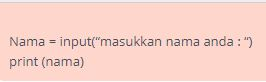
\includegraphics[width=4cm]{figures/1184030/inputpy2.png}
			\centering
			\caption{input pada python 2}
			\end{figure}
		Pada Python 3, Sintaks yang digunakan untuk mencetak inputan yang digunakan yaitu : 
		\hfill \break
			\begin{figure}[H]
			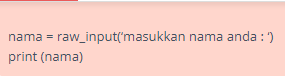
\includegraphics[width=4cm]{figures/1184030/inputpy3.png}
			\centering
			\caption{input pada python 3}
			\end{figure}
		\item Sintaks yang digunakan dan hasil ketika melakukan operator pembagian\\
	\begin{enumerate}
	\item Berikut ini sintaks pembagian yang dituliskan melalui python 2 :
		\hfill \break
			\begin{figure}[H]
			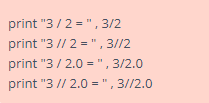
\includegraphics[width=4cm]{figures/1184030/bagipy2.png}
			\centering
			\caption{sintaks operasi pembagian di python 2}
			\end{figure}
		Melalui sintaks tersebut didapatkan hasil seperti berikut :
		\hfill \break
			\begin{figure}[H]
			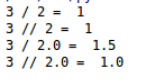
\includegraphics[width=4cm]{figures/1184030/hbpy2.png}
			\centering
			\caption{hasil dari operasi pembagian di python 2}
			\end{figure}
	\item Berikut ini sintaks pembagian yang dituliskan melalui python 3 :
		\hfill \break
			\begin{figure}[H]
			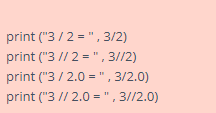
\includegraphics[width=4cm]{figures/1184030/bagipy3.png}
			\centering
			\caption{sintaks operasi pembagian di python 3}
			\end{figure}
		Melalui sintaks yang dituliskan tersebut didapatkan hasil seperti berikut :
		\hfill \break
			\begin{figure}[H]
			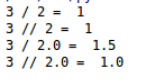
\includegraphics[width=4cm]{figures/1184030/hbpy2.png}
			\centering
			\caption{hasil dari operasi pembagian di python 3}
			\end{figure}
	\end{enumerate}			
\end{itemize}
	\item Implementasi Python dan Penggunaan di Perusahaan Kelas Dunia\\
	Dalam penggunaannya, Python diklaim sebagai bahasa skrip yang menggabungkan kemampuan atau kapabilitas dan sintaksis kode yang sangat jelas. Selain itu, python juga dilengkapi dengan fungsionalitas standar yang besar serta komprehensif. Oleh karenanya, python banyak digunakan oleh perusahaan-perusahaan besar skala nasional maupun internasional.\\
	Berikut ini merupakan beberapa dari banyaknya perusahaan yang menggunakan Python dalam pengembangan usaha mereka, di antaranya yaitu :
	\begin{enumerate}
		\item Instagram
		\item Google
		\item Quora
		\item Spotify
		\item Netflix
		\item Facebook
	\end{enumerate}
\section{Instalasi}
\begin{itemize}
	\item Instalasi Python\\
	Berikut merupakan urutan yang dilakukan saat melakukan instalasi python, di antaranya yaitu :\\
	\begin{enumerate}
		\item Klik icon Anaconda kemudian klik install atau setup. Setelah itu klik next.
		\begin{figure}[H]
			\includegraphics[width=4cm]{figures/1184030/anaconda/1.png}
			\centering
			\caption{setup anaconda}
			\end{figure}
		\item Setelah itu, klik I agree pada licence agreement.\\
			\begin{figure}[H]
			\includegraphics[width=4cm]{figures/1184030/anaconda/2.png}
			\centering
			\caption{licence agreement}
			\end{figure}
		\item Pilih All User pada installation type, hal ini memungkinkan agar anaconda dapat digunakan oleh semua user pada PC.\\
			\begin{figure}[H]
			\includegraphics[width=4cm]{figures/1184030/anaconda/3.png}
			\centering
			\caption{installation type}
			\end{figure}
		\item Pilih lokasi penyimpanan aplikasi Anaconda yang akan diinstal, kemudian klik next.\\
			\begin{figure}[H]
			\includegraphics[width=4cm]{figures/1184030/anaconda/4.png}
			\centering
			\caption{lokasi penyimpanan anaconda}
			\end{figure}
		\item Ceklis bagian ADD Environtment to the Path, hal ini memungkinkan untuk menambahkan environtment anaconda ke dalam path yang ada dalam PC anda. Setelah itu klik next.
			\begin{figure}[H]
			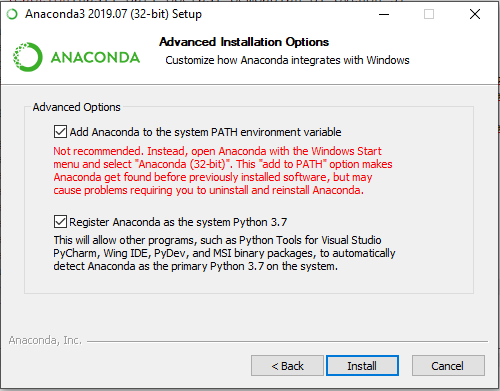
\includegraphics[width=4cm]{figures/1184030/anaconda/5PNG.png}
			\centering
			\caption{menambahkan path environtment}
			\end{figure}
		\item Tunggu sampai instalasi selesai.
			\begin{figure}[H]
			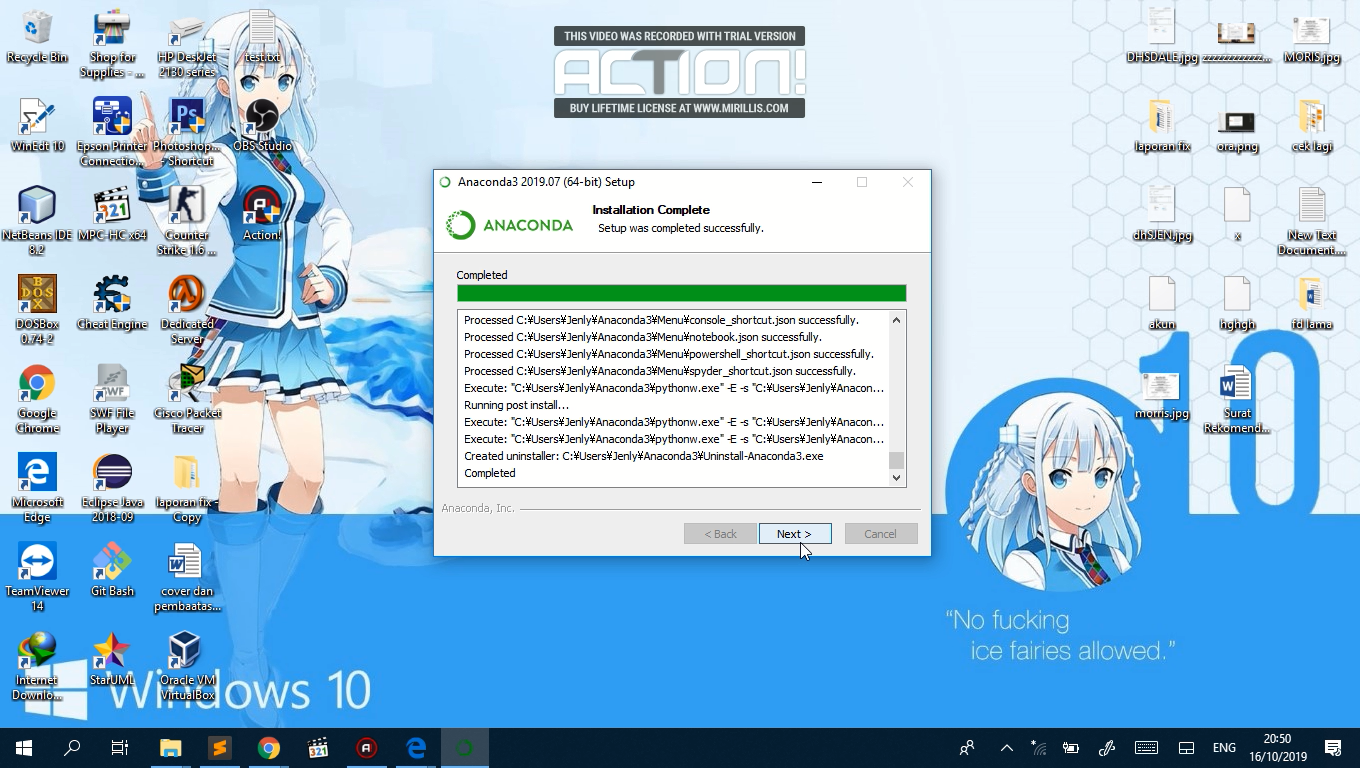
\includegraphics[width=4cm]{figures/1184030/anaconda/7.png}
			\centering
			\caption{proses instalasi}
			\end{figure}
		\item Setelah Instalasi selesai, maka klik next sampai proses terakhir dan klik finish di akhir proses instalasi seperti pada gambar berikut ini.\\
			\begin{figure}[H]
			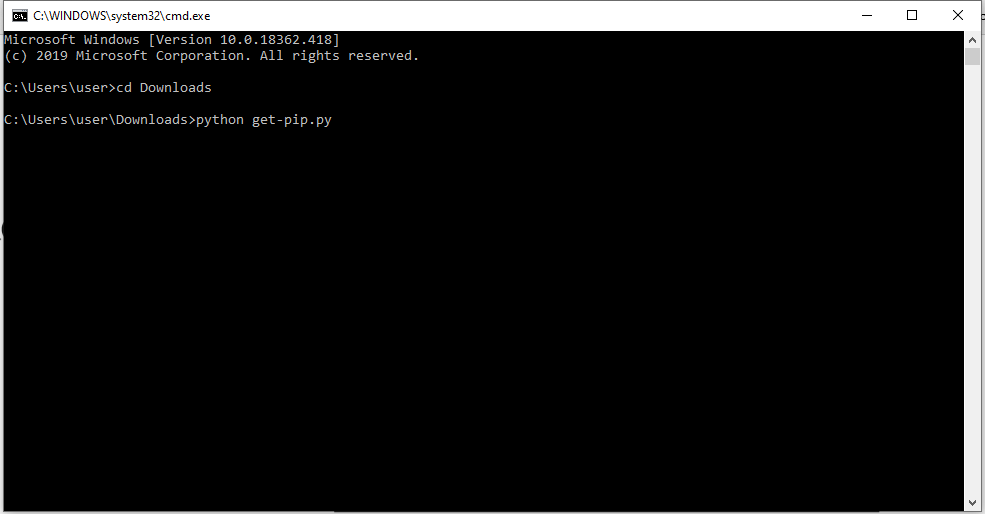
\includegraphics[width=4cm]{figures/1184030/anaconda/8.png}
			\centering
			\caption{instalasi selesai}
			\end{figure}
			\begin{figure}[H]
			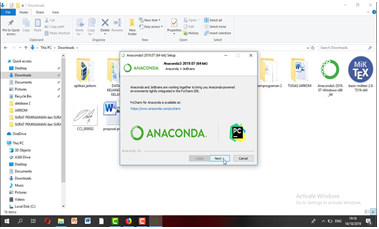
\includegraphics[width=4cm]{figures/1184030/anaconda/9.png}
			\centering
			\caption{instalasi selesai 2}
			\end{figure}
			\begin{figure}[H]
			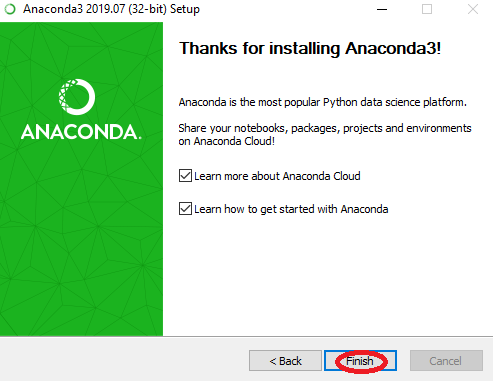
\includegraphics[width=4cm]{figures/1184030/anaconda/10.png}
			\centering
			\caption{instalasi selesai 3}
			\end{figure}
	\end{enumerate}
	\item Instalasi PIP
		PIP umumnya sudah terinstal di dalam Environtment secara otomatis ketika kita sudah menginstall Python maupun melalui Navigator Anaconda. Langkah awal yang dilakukan untuk menginstalasi PIP yaitu :
		\begin{enumerate}
			\item Buka command prompt lalu ketikkan "pip --version", hal ini dilakukan untuk memastikan bahwa pip telah terinstal dalam PC ataupun belum. Lihatlah contoh gambar di bawah ini
				\begin{figure}[H]
				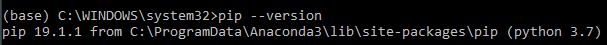
\includegraphics[width=8cm]{figures/1184030/pip/cekpip.png}
				\centering
				\caption{mengecek versi pip yang terinstal di pc}
				\end{figure}
			\item Download dan update versi pip terbarunya dengan mendownload package dari cmd. Hal ini bisa dilakukan dengan beberapa cara, di antaranya :
			\begin{enumerate}
				\item Ketikkan "curl https://bootstrap.pypa.io/get-pip.py -o get-pip.py". Hasil yang akan didapatkan dapat dilihat seperti gambar berikut ini :
				\begin{figure}[H]
				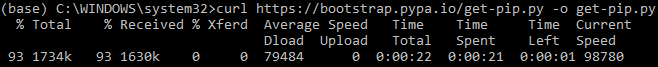
\includegraphics[width=8cm]{figures/1184030/pip/downloadpip.png}
				\centering
				\caption{mendownload pakage pip yang ada}
				\end{figure}
				\item Menggunakan ketikan "pip install -U pip"
				\begin{figure}[H]
				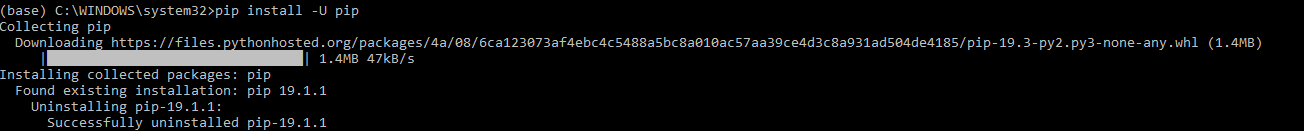
\includegraphics[width=8cm]{figures/1184030/pip/upgrdpip.png}
				\centering
				\caption{mendownload dan mengupgrade versi pip}
				\end{figure}
				\item Dengan mengetikkan "python -m pip install --upgrade pip"
				\begin{figure}[H]
				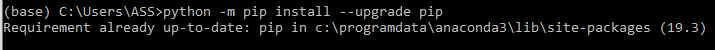
\includegraphics[width=8cm]{figures/1184030/pip/upgrd3.png}
				\centering
				\caption{mendownload dan mengupgrade versi pip 2}
				\end{figure}
			\end{enumerate}
			\item Cek kembali versi pip dengan mengetikkan sintaks "pip --version" pada cmd. Setelah itu lihat hasilnya, apakah terdapat perubahan ataukah tidak.
				\begin{figure}[H]
				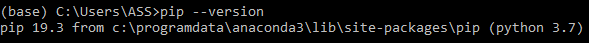
\includegraphics[width=8cm]{figures/1184030/pip/cekver.png}
				\centering
				\caption{mendownload dan mengupgrade versi pip}
				\end{figure}
		\end{enumerate}
	\item Setting Environtment
		\begin{enumerate}
			\item Buka control panel
				\begin{figure}[H]
				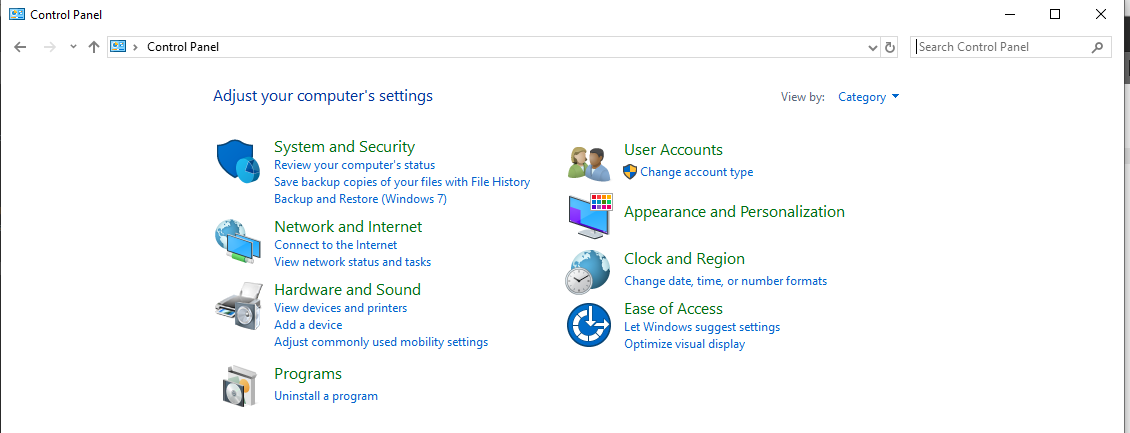
\includegraphics[width=8cm]{figures/1184030/environtment/control.png}
				\centering
				\caption{update anaconda}
				\end{figure}
			\item Pilih System and Security
				\begin{figure}[H]
				\includegraphics[width=8cm]{figures/1184030/environtment/2.png}
				\centering
				\caption{update anaconda}
				\end{figure}
			\item Kemudian pilih System
				\begin{figure}[H]
				\includegraphics[width=8cm]{figures/1184030/environtment/3.png}
				\centering
				\caption{update anaconda}
				\end{figure}
			\item Pilih Advance System Settings
				\begin{figure}[H]
				\includegraphics[width=8cm]{figures/1184030/environtment/4.png}
				\centering
				\caption{advance system settings}
				\end{figure}
			\item Pada bagian Advance, pilih Environtment Variable untuk menyunting environtment
				\begin{figure}[H]
				\includegraphics[width=8cm]{figures/1184030/environtment/3.png}
				\centering
				\caption{edit environtment variable}
				\end{figure}
		\end{enumerate}
	\item Mencoba Entrepeter/CLI melalui terminal atau windows
		\begin{enumerate}
			\item Buka cmd kemudian ketikkan python
				\begin{figure}[H]
				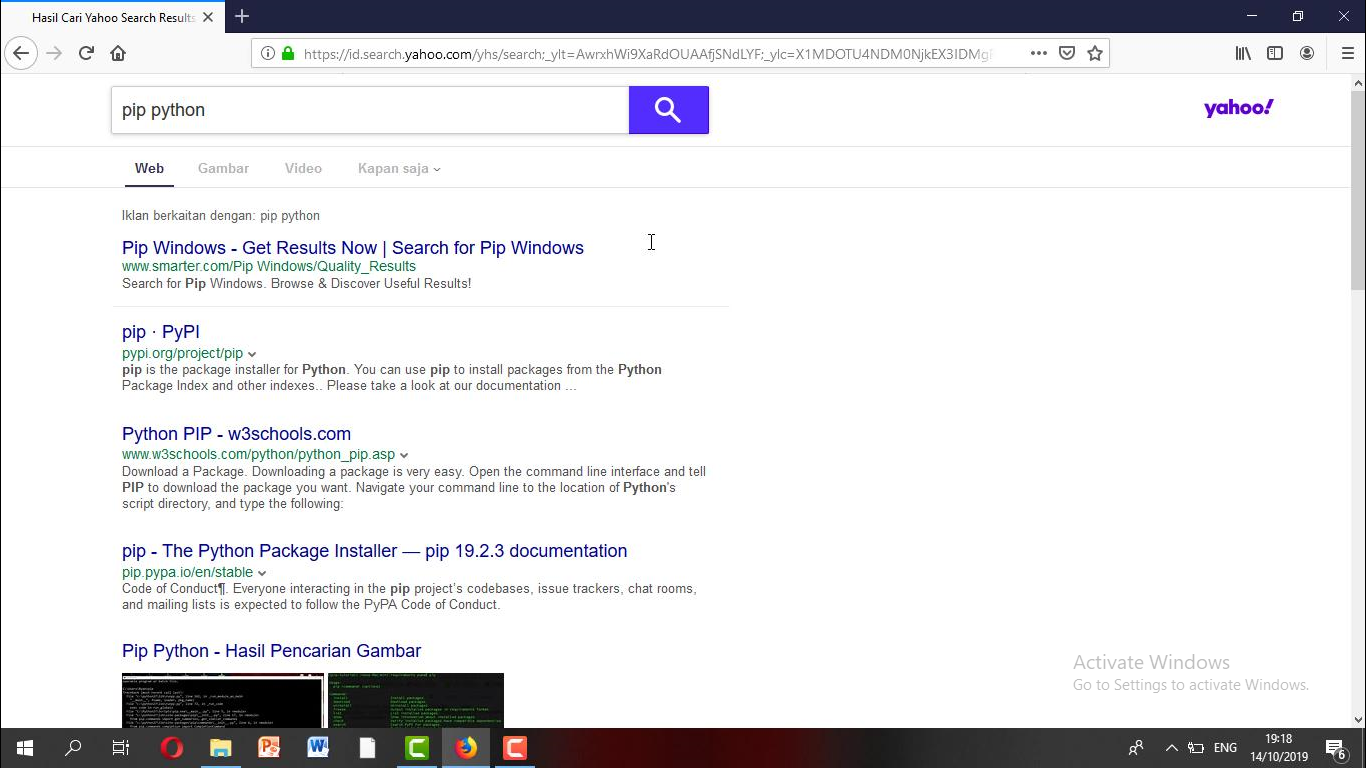
\includegraphics[width=8cm]{figures/1184030/interpreter/11.png}
				\centering
				\caption{tampilan awal cmd setelah diketik "python"}
				\end{figure}
			\item ketikkan exit()
				\begin{figure}[H]
				\includegraphics[width=8cm]{figures/1184030/interpreter/2.png}
				\centering
				\caption{untuk keluar dari environtmen terlebih dahulu sebelum mengaktifkan conda environtment}
				\end{figure}
			\item aktifkan conda environtment dengan mengetikkan "conda activate"
				\begin{figure}[H]
				\includegraphics[width=8cm]{figures/1184030/interpreter/3.png}
				\centering
				\caption{mengaktifkan conda environtment}
				\end{figure}
			\item ketikkan python kembali sehingga tampilan akan berubah seperti gambar di bawah ini
				\begin{figure}[H]
				\includegraphics[width=8cm]{figures/1184030/interpreter/1.png}
				\centering
				\caption{tampilan setelah conda environtment diaktifkan}
				\end{figure}
			\item ketikkan beberapa sintaks untuk mencoba enterpreter. Disini saya menggunakan sintaks untuk mencetak atau print
				\begin{figure}[H]
				\includegraphics[width=8cm]{figures/1184030/interpreter/4.png}
				\centering
				\caption{hasil mencoba enterpreter di cmd}
				\end{figure}
		\end{enumerate}
	\item Menjalankan dan mengupdate anaconda dan spyder
		Anaconda dan spyder merupakan satu kesatuan karena di dalam navigator anaconda terdapat IDE Spyder. Oleh karenanya dengan mengupdate anacondanya, maka spyder juga otomatis terupdate. Berikut ini merupakan tata cara untuk mengupdate anaconda, di antaranya adalah :
		\begin{enumerate}
			\item buka cmd atau dapat juga melalui Anaconda Prompt
			\item untuk memulai menggunakan cmd, ketikkan python terlebih dahulu
			\item Setelah itu ketikkan exit() untuk keluar dari conda environtment
			\item Ketikkan conda activate untuk mengaktifkan conda environtment
			\item Untuk memulai dengan Anaconda prompt anda bisa langsung ke tahap ini, yakni ketikkan "conda install -c anaconda python" seperti gambar berikut ini
				\begin{figure}[H]
				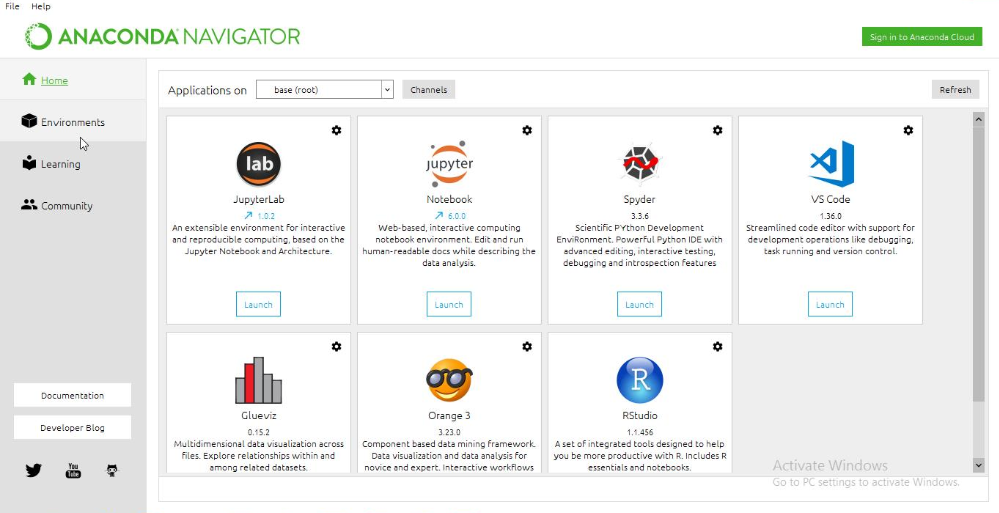
\includegraphics[width=8cm]{figures/1184030/anaconda/update1.png}
				\centering
				\caption{install update anaconda}
				\end{figure}
				Setelah proses seperti gambar di atas berjalan, lalu ketikkan "Y" untuk melanjutkan proses seperti gambar 						berikut
				\begin{figure}[H]
				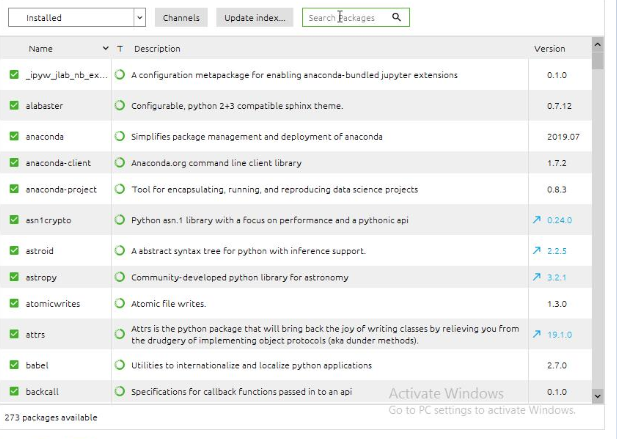
\includegraphics[width=8cm]{figures/1184030/anaconda/update2.png}
				\centering
				\caption{konfirmasi update}
				\end{figure}
		\end{enumerate}
	\item Menjalankan script "Hello World" di Spyder
	 Berikut ini merupakan cara untuk menjalankan script "Hello World", di antaranya yaitu :
	 \begin{enumerate}
	 	\item Buka spyder melalui navigator anaconda yang telah diinstall sebelumnya.
	 		\begin{figure}[H]
			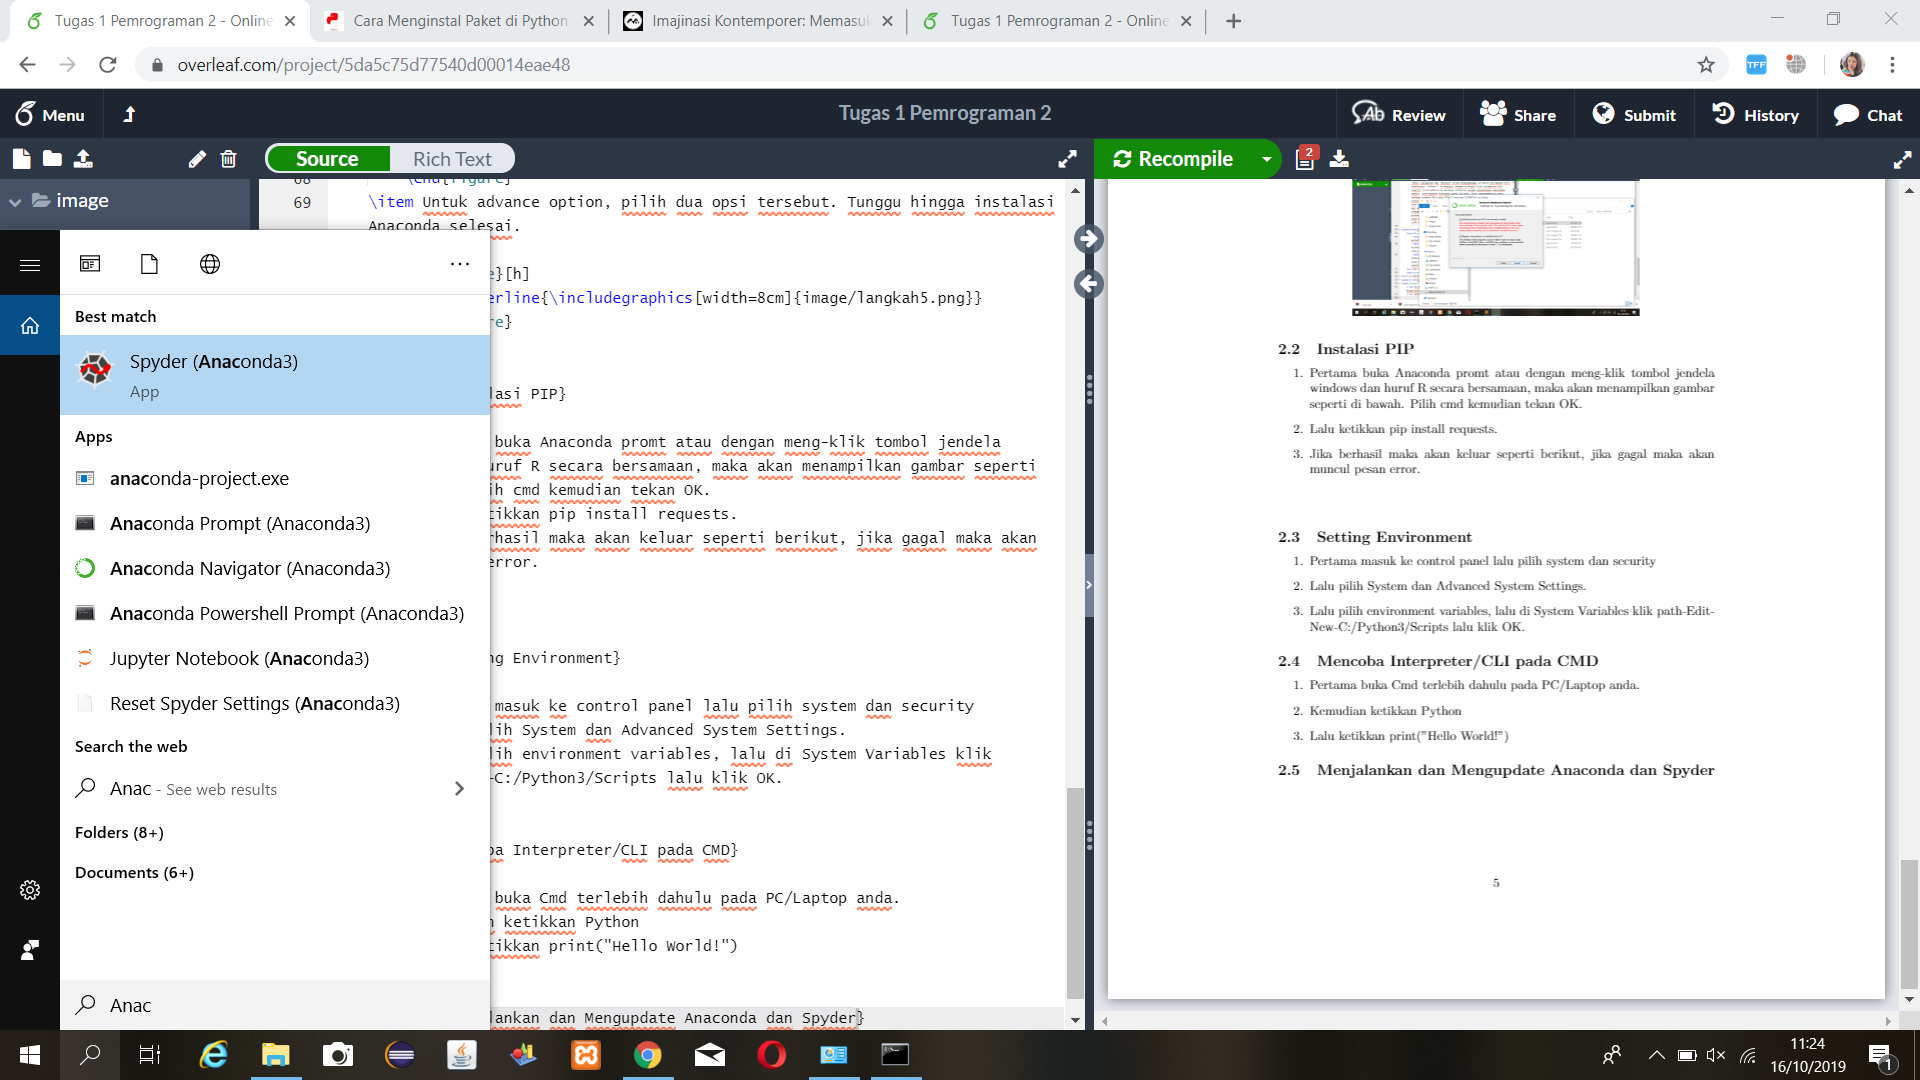
\includegraphics[width=8cm]{figures/1184030/spyder.png}
			\centering
			\caption{tampilan spyder}
			\end{figure}
	 	\item Tuliskan script yang akan dibuat
	 		\begin{figure}[H]
			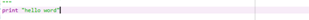
\includegraphics[width=8cm]{figures/1184030/hello.png}
			\centering
			\caption{script hello world}
			\end{figure}
	 	\item Tekan tombol run untuk menjalankan script yang telah dibuat sebelumnya. Setelah itu pada iPython akan menampilkan teks "Hello World"
	 		\begin{figure}[H]
			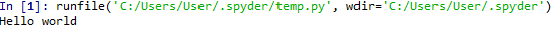
\includegraphics[width=8cm]{figures/1184030/hasil.png}
			\centering
			\caption{tampilan hasil}
			\end{figure}
	 \end{enumerate}
	\item Menjalankan script otomatis login aplikasi akademik dengan library selenium dan inputan user
		Untuk menjalankan script otomatis login dengan library selenium diperlukan tahapan sebagai berikut :
		\begin{enumerate}
		\item Buka command prompt kemudian ketikkan "pip install selenium" untuk menginstall paket library selenium ke pc kita
			\begin{figure}[H]
			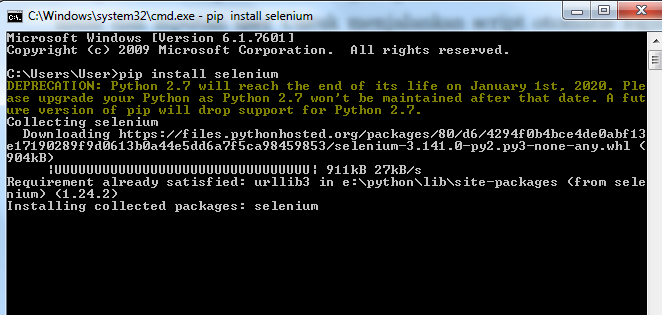
\includegraphics[width=8cm]{figures/1184030/selenium.png}
			\centering
			\caption{install selenium}
			\end{figure}
		\item Download geckodriver.exe sesuai versi yang dibutuhkan oleh pc anda
		\item Letakkan geckodriver.exe tersebut ke dalam system32 yang ada di dalam local disk c
		\item Buka IDE Spyder untuk menuliskan script
			\begin{figure}[H]
			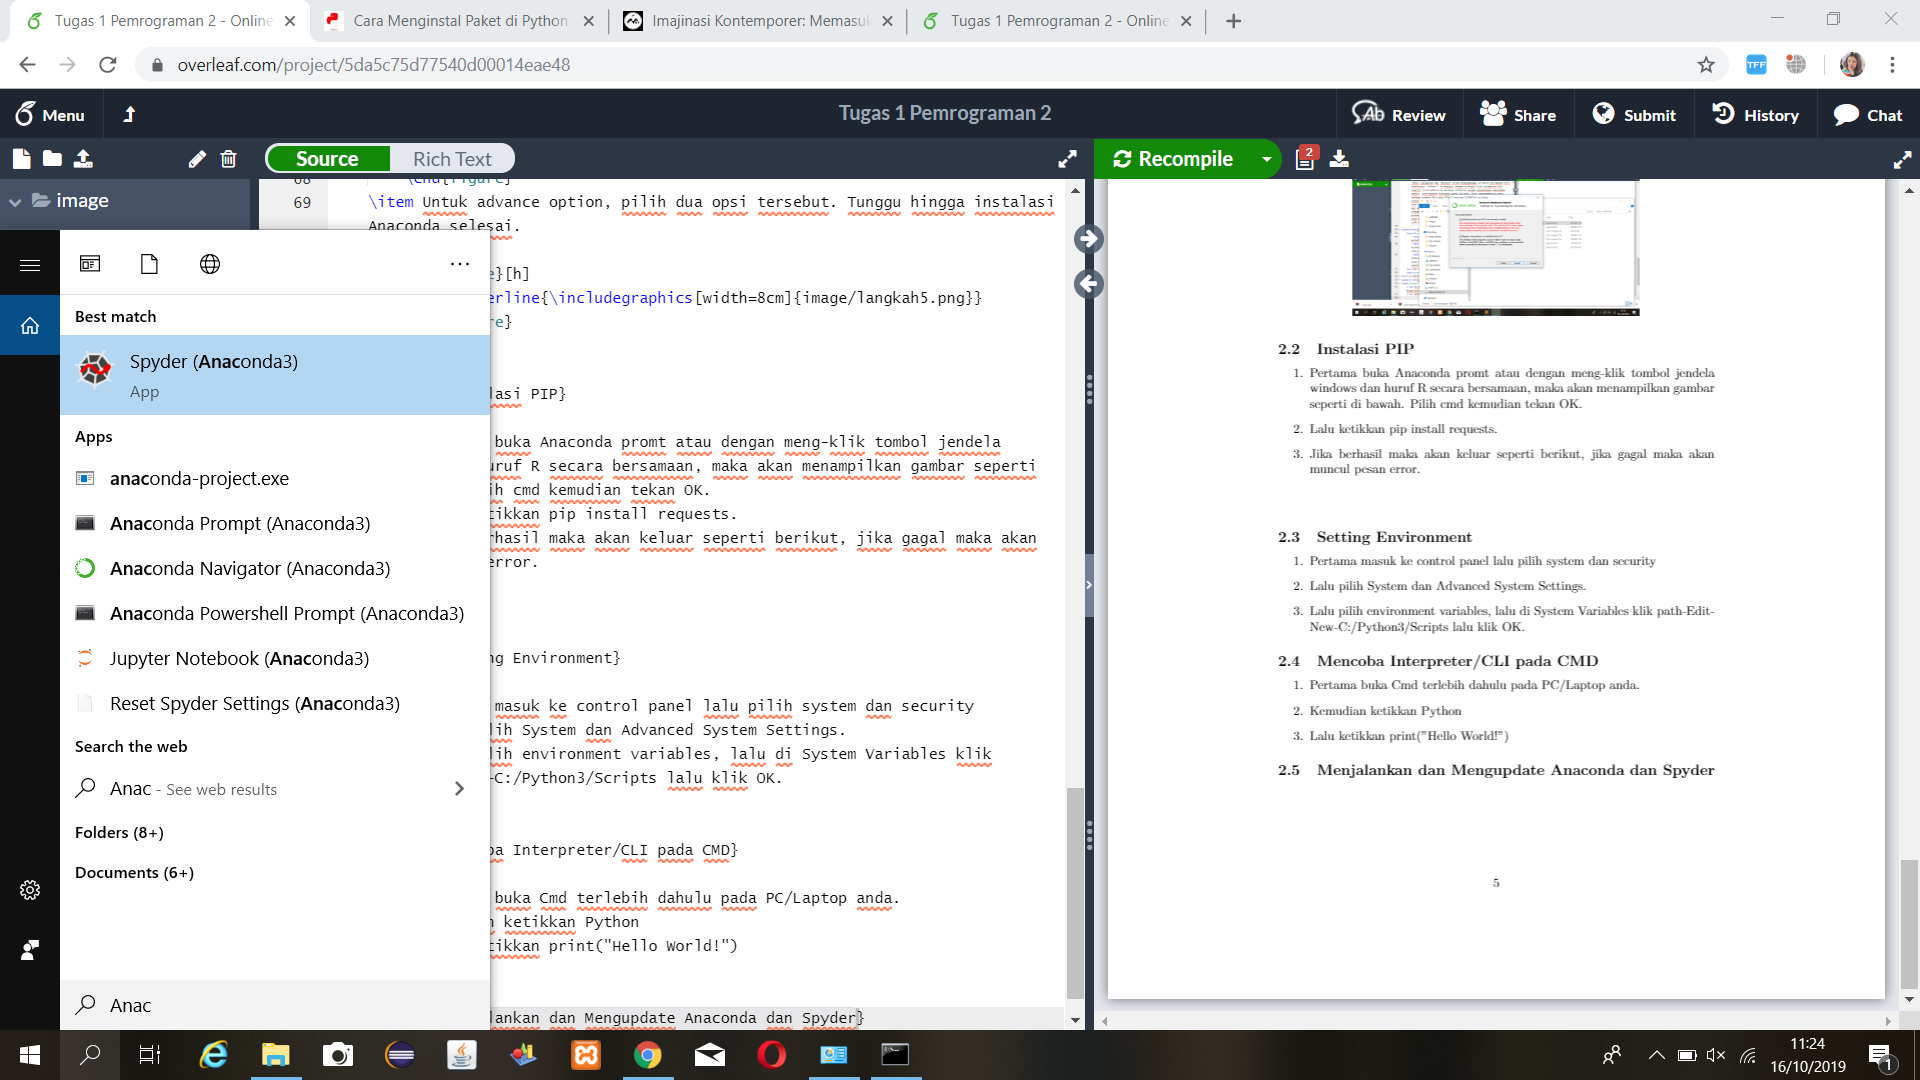
\includegraphics[width=8cm]{figures/1184030/spyder.png}
			\centering
			\caption{tampilan spyder}
			\end{figure}
		\item Tuliskan script perintah selenium yang akan dijalankan. Berikut script yang dituliskan :
			\begin{figure}[H]
			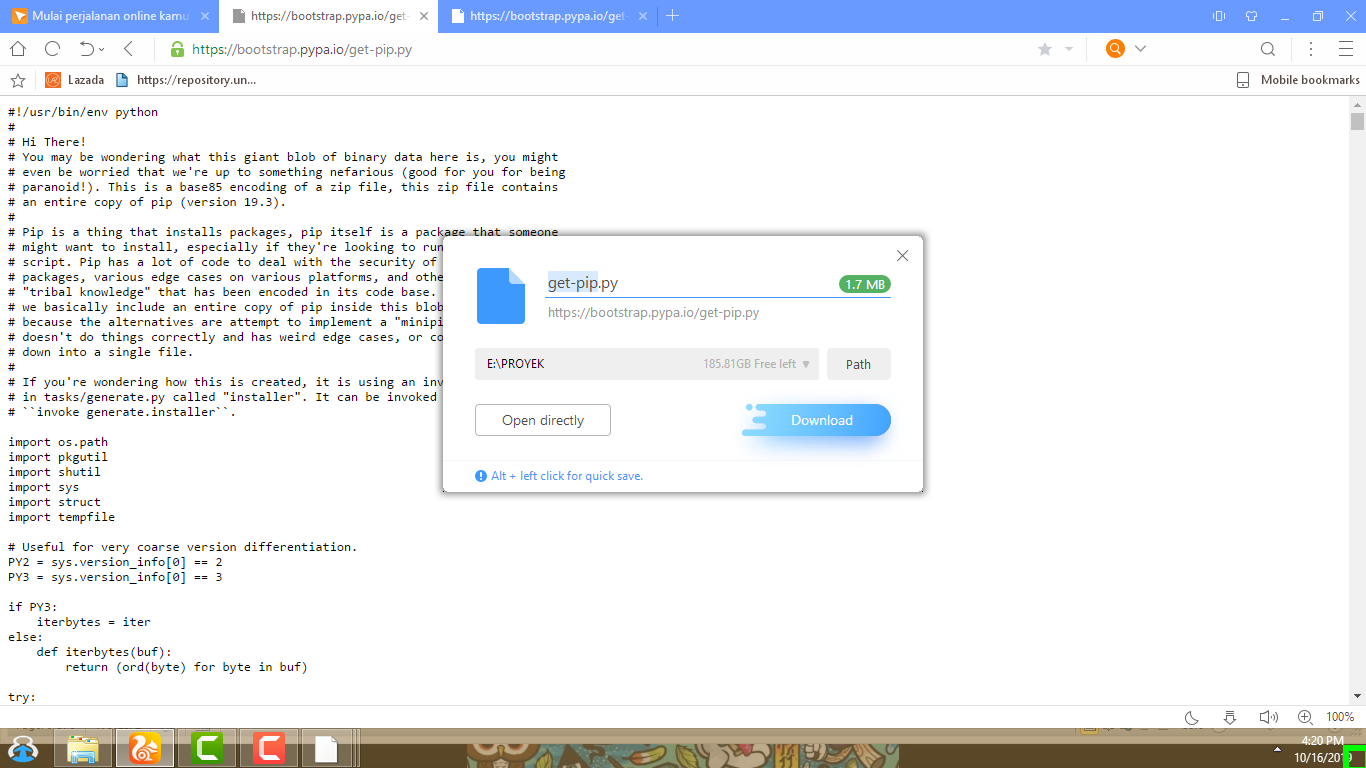
\includegraphics[width=8cm]{figures/1184030/20.png}
			\centering
			\caption{kode script login otomatis}
			\end{figure}
		\item Halaman akan otomatis masuk ke sistem akademik siap dengan menginputkan username dan email yang sesuai dalam script yang telah ditulis sebelumnya
			\begin{figure}[H]
			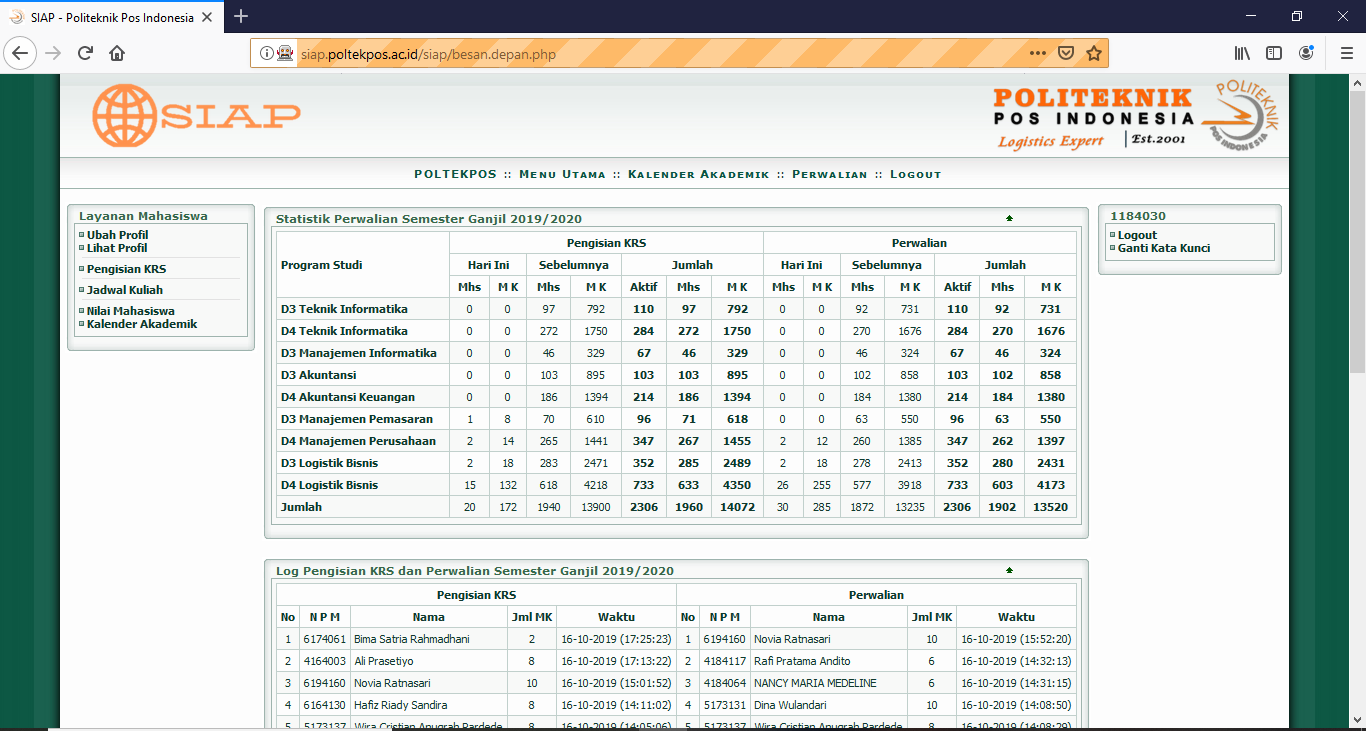
\includegraphics[width=8cm]{figures/1184030/siap.png}
			\centering
			\caption{login otomatis ke sistem akademik siap}
			\end{figure}
		\end{enumerate}
		\item Memakai Variable Explorer di Spyder
		\begin{enumerate}
		\item Tulis kode script pada spyder berupa variabel
			\begin{figure}[H]
			\includegraphics[width=8cm]{figures/1184030/variabel/1.png}
			\centering
			\caption{penulisan variabel}
			\end{figure}
		\item Run kode tersebut, maka nama, tipe, dan nilai akan keluar di variabel explorer
			\begin{figure}[H]
			\includegraphics[width=8cm]{figures/1184030/variabel/2.png}
			\centering
			\caption{tampilan variabel explorer}
			\end{figure}
		\item Pada ipython console akan tertera hasil dari script yang diketik sebelumnya
			\begin{figure}[H]
			\includegraphics[width=8cm]{figures/1184030/variabel/3.png}
			\centering
			\caption{console dari script yang dibuat}
			\end{figure}
		\item Untuk mengedit variabel yang telah dibuat sebelumnya, klik kanan pada variabel explorer. Maka akan dimunculkan tampilan seperti berikut ini
			\begin{figure}[H]
			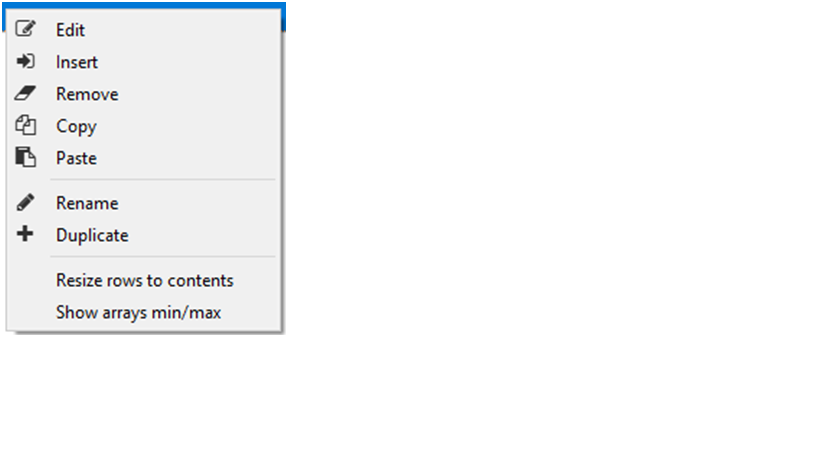
\includegraphics[width=8cm]{figures/1184030/variabel/4.png}
			\centering
			\caption{edit variabel}
			\end{figure}
		\end{enumerate}
\end{itemize}
\section{Identasi}
\begin{itemize}
	\item Penjelasan Identasi
		Indentasi berasal dari bahasa Inggris Indentation yang bermakna menggeser atau men'jorok'kan ke dalam. Hal itu maksudnya bahwa menjorokkan script kode ke dalam merupakan indentasi. Indentasi di dalam bahasa python digunakan sebagai penanda blok program, sedangkan pada umumnya indentasi digunakan untuk mempermudah dalam membaca script kode yang telah dibuat. Oleh karenanya, indentasi di dalam script python sangatlah penting dan bisa menyebabkan error jika kita tidak menggunakannya.
	\item Jenis-jenis error identasi yang didapat
			Jenis error indentasi yag dapat terjadi ada 12 keadaan dalam bahasa pemrograman yang berbeda-beda. Pada bahasa pemrograman python, jenis error indentasi yang terjadi adalah ketika kita salah atau tidak memberi identasi atau menjorok pada script. Hal itu dikarenakan pada python, indentasi adalah penanda blok program.
	\item Cara membaca error yang ada pada identasi
	\begin{enumerate}
	\item Lihat pada jendela script. Jika terdapat tanda warning atau tanda silang, maka hal itu menandakan bahwa terdapat error pada script yang anda buat
			\begin{figure}[H]
			\includegraphics[width=8cm]{figures/1184030/error/1.png}
			\centering
			\caption{error indentasi}
			\end{figure}
	\item Selain itu, lihat pada jendela iPython Console. Jika terdapat error maka saat script dijalankan maka akan menampilkan warning seperti berikut
			\begin{figure}[H]
			\includegraphics[width=8cm]{figures/1184030/error/2.png}
			\centering
			\caption{error indentasi pada console}
			\end{figure}
	\end{enumerate}
	\item Cara menangani error yang terjadi
	\begin{enumerate}
		\item Cek ke baris yang dituju, yakni baris yang terdapat tanda warning seperti gambar tersebut
			\begin{figure}[H]
			\includegraphics[width=8cm]{figures/1184030/error/1.png}
			\centering
			\caption{error indentasi pada console}
			\end{figure}
		\item Perhatikan Warning kesalahan yang muncul pada jendela iPython Console terhadap baris tersebut
			\begin{figure}[H]
			\includegraphics[width=8cm]{figures/1184030/error/2.png}
			\centering
			\caption{error indentasi pada console}
			\end{figure}
		\item Setelah itu perbaiki kesalahan yang terjadi sehingga tanda warning pada line tersebut menghilang
			\begin{figure}[H]
			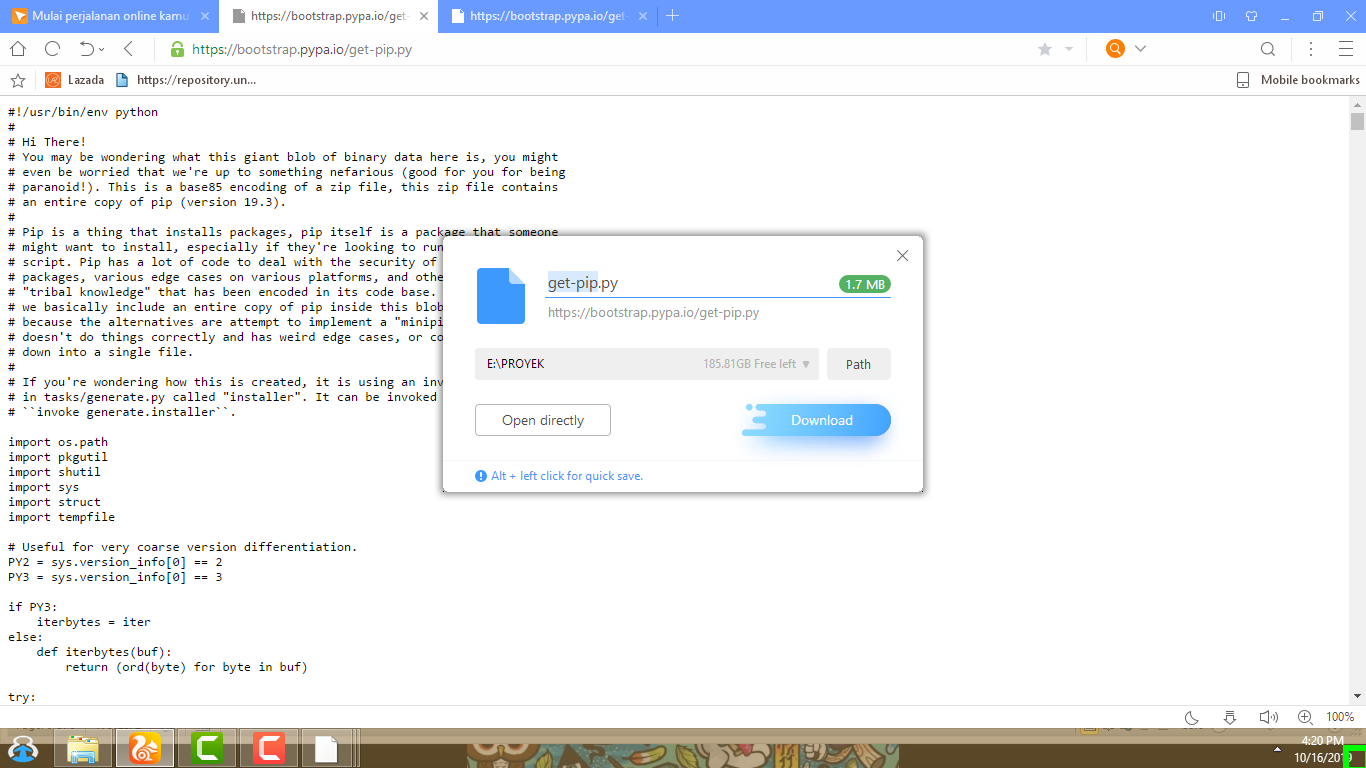
\includegraphics[width=8cm]{figures/1184030/20.png}
			\centering
			\caption{error yang telah diperbaiki}
			\end{figure}
		\item Run kembali script yang dituju
	\end{enumerate}
\end{itemize}
